\documentclass[12pt]{book}
\usepackage[italian]{babel} % a capo in ita
\usepackage{amsmath}
\usepackage{amsfonts} 
\usepackage{amssymb}
\usepackage{graphicx}
\usepackage{listings}
\usepackage {xcolor}
\usepackage {color}
\graphicspath{ {./Immagini/} }
\usepackage{float}

\definecolor{lightyellow}{rgb}{1, 1, 0.7}
\lstset{ %
	language=C++,                % choose the language of the code
	basicstyle=\footnotesize,       % the size of the fonts that are used for the code
	numbers=left,                   % where to put the line-numbers
	numberstyle=\footnotesize,      % the size of the fonts that are used for the line-numbers
	stepnumber=1,                   % the step between two line-numbers. If it is 1 each line will be numbered
	numbersep=5pt,                  % how far the line-numbers are from the code
	backgroundcolor=\color{lightyellow},  % choose the background color. You must add \usepackage{color}
	showspaces=false,               % show spaces adding particular underscores
	showstringspaces=false,         % underline spaces within strings
	showtabs=false,                 % show tabs within strings adding particular underscores
	frame=single,           % adds a frame around the code
	tabsize=2,          % sets default tabsize to 2 spaces
	captionpos=b,           % sets the caption-position to bottom
	breaklines=true,        % sets automatic line breaking
	breakatwhitespace=false,    % sets if automatic breaks should only happen at whitespace
	escapeinside={(*}{*)},%         % if you want to add a comment within your code
}

\huge
\title{Guida a CustomGraphics}
\author{3ªCET}
\date{Anno Scolastico 2022-2023}


\begin{document}  
	\maketitle 
	\tableofcontents
	
	\newpage
	\section{Introduzione}
	CustomGraphics è una libreria che integra diverse istruzioni per la programmazione grafica.
	E' presente all'interno del template "Pino10".
	
	
	\chapter{Istruzioni}
		\section{GraphicScanfXY}
		L'istruzione "graphicscanfxy" viene usata per acquisire un dato da parte dell'utente. Questo valore, che può essere di tipo int, di tipo float o di tipo char, viene poi inserito all'interno di una variabile dichiarata in precedenza. In un ambiente di programmazione grafica non è possibile usare il comando "scanf", che viene invece usato in ambienti testuali.
		\\La sintassi è la seguente:
		\\
		\\
		\Large graphicScanfxy(x, y, "formato", \&var);
		\normalsize
		\\
		\\- x: indica la coordinata x del punto nel quale l'utente inserirà un valore;
		\\- y: indica la coordinata y del punto nel quale l'utente inserirà un valore;
		\\- "formato": indica il formato della variabile che si vuole acquisire ("\%f"= float "\%d"= int);
		\\- var: il nome della variabile nella quale inserire il valore acquisito;
		\\- center: indica il centro del diagramma cartesiano disegnato con la funzione assi (Bisogna inserire lo stesso valore inserito nella funzione assi);
		\newpage
		%	------------------------------------------
		\section{Assi}
			L'istruzione "assi" viene usata per visualizzare sullo schermo un diagramma cartesiano, da usare come base per tracciare grafici e diagrammi.
			\\La sintassi è la seguente:
			\\\\
			\Large assi(rx, ry, center);\\
			\normalsize
			\\- rx: il numero di parti in cui è diviso l'asse delle ascisse (con rx=40 si ottiene un grafico che va da 	x=-20 a x=20);
			\\- ry: il numero di parti in cui è diviso l'asse delle ordinate, in maniera analoga ad rx;
			\\- center: indica la tipologia di grafico da disegnare: center=1 corrisponde ad un grafico con l'origine al centro della finestra, qualunque altro numero genera un grafico in cui l'origine è situata nell'angolo in basso a sinistra.
			\\
			\\ Questo programma genera un piano cartesiano che spazia da -10 a 10 nelle ascisse e da -30 a 30 nelle ordinate, con l'origine posta al centro della finestra.
			\\ \\Codice:
			\begin{lstlisting}
	{
		initwindow(850, 610);	
		assi(20, 60, 1);	
		getch();
	}
			\end{lstlisting}
			\newpage
			Output:
			\begin{figure}[h]
				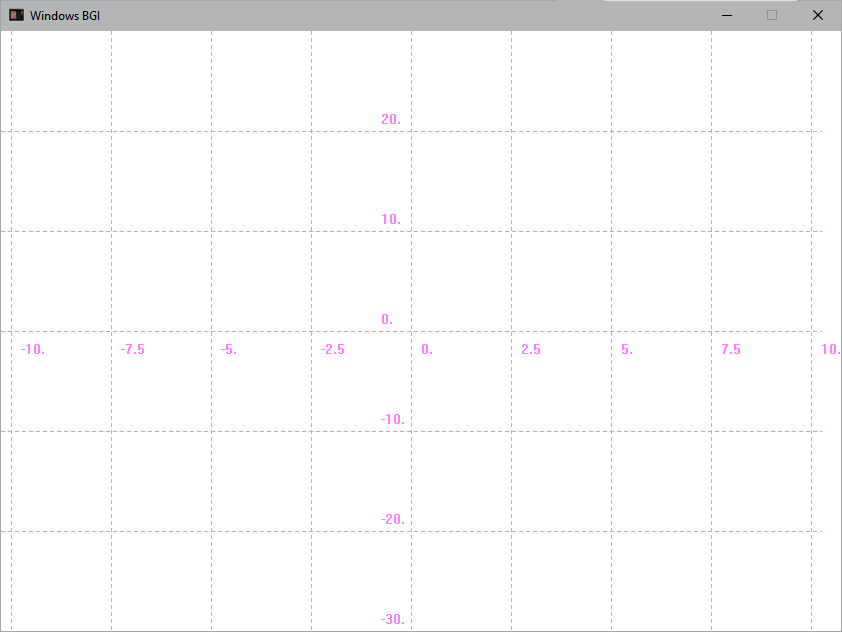
\includegraphics[scale=0.5]{assiterminale1}
			\end{figure}
		\newpage
	
%	------------------------------------------

		\section{TracciaPixel}
			L'istruzione "tracciapixel" viene usata per visualizzare un pixel, di posizione e colore a scelta, all'interno della finestra.
			\\La sintassi è la seguente:
			\\
			\\
			\Large tracciapixel(x, y, rx, ry, col, center);
			\normalsize
			\\
			\\- x: indica la coordinata x del punto che si vuole tracciare sullo schermo;
			\\- y: coordinata y del punto che si vuole tracciare sullo schermo;
			\\- rx: Il numero di parti in cui è diviso l'asse delle ascisse (Bisogna inserire lo stesso valore inserito nella funzione assi);
			\\- ry:Il numero di parti in cui è diviso l'asse delle ordinate(Bisogna inserire lo stesso valore inserito nella funzione assi);
			\\- col: indica il colore del pixel.
			\\- center: indica il centro del diagramma cartesiano disegnato con la funzione assi (Bisogna inserire lo stesso valore inserito nella funzione assi);
			
			
			Questo programma colora un singolo pixel su un diagramma cartesiano, dopo aver ottenuto le coordinate di esso tramite l'uso di "graphicScanfxy". Inoltre usa "cleardevice" per "ripulire" lo schermo. E' difficile da notare, ma a coordinate (4,7) è presente un pixel colorato di rosso.
		\newpage Codice e output:\\			
		\begin{lstlisting}
			{
				initwindow(850, 610);
				float x, y;
				
				outtextxy(50, 50, "Inserisci x:");
				graphicScanfxy(300, 50, "%f", &x);
				outtextxy(50, 100, "Inserisci y:");
				graphicScanfxy(300, 100, "%f", &y);
				cleardevice();
				
				int rx, ry;
				rx = 40;
				ry = 60;
				assi(rx, ry, 1);
				
				tracciapixel(x,y,rx,ry,4,1);
				getch();
			}
		\end{lstlisting}
		
		
		\begin{figure*}[h]
			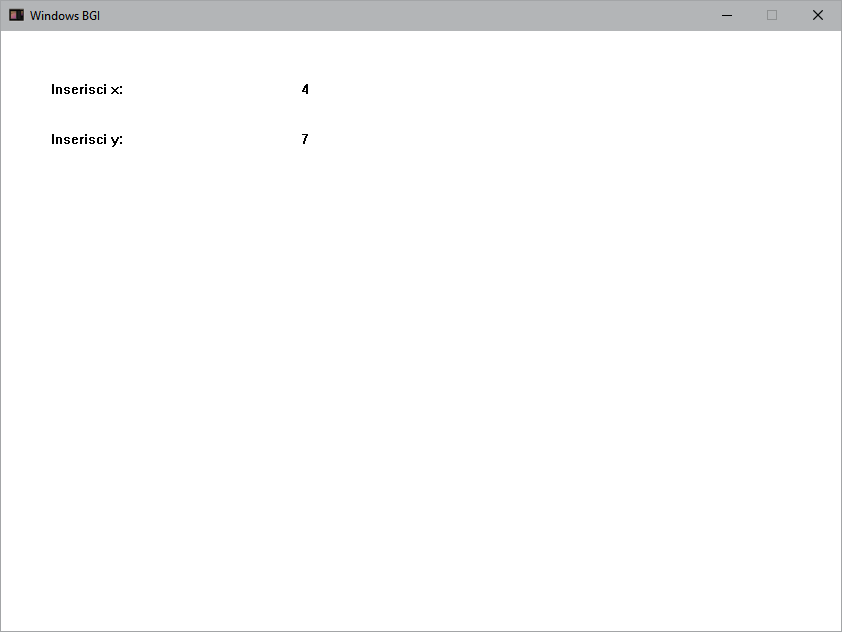
\includegraphics[scale=0.5]{tracciapixelterminale1}
				\\ \\
			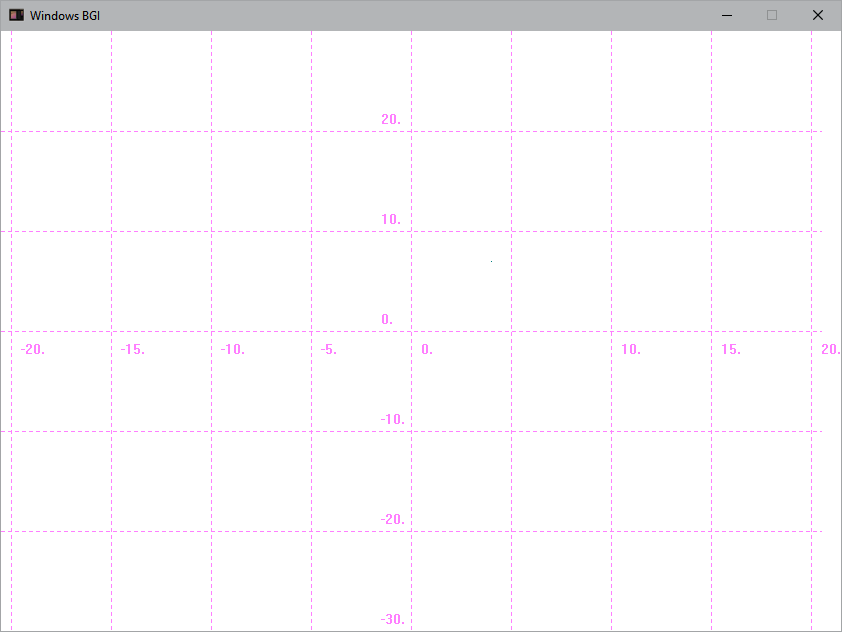
\includegraphics[scale=0.5]{tracciapixelterminale2}
		\end{figure*}
		\clearpage
		\newpage
		
		\newpage
%	------------------------------------------
		
		\section{TracciaRetta}
			L'istruzione "tracciaretta" viene usata per creare una linea retta di pixel, di colore a scelta, per visualizzare una retta all'interno della finestra. Viene usata insieme al comando "assi" per creare grafici.
			\\La sintassi è la seguente:
			\\
			\\
			\Large tracciaretta(m, q, rx, ry, col, center);
			\normalsize
			\\
			\\- m: indica il coefficiente angolare della retta da rappresentare
			\\- y: indica la quota della retta da rappresentare;
			\\- rx: Il numero di parti in cui è diviso l'asse delle ascisse (Bisogna inserire lo stesso valore inserito nella funzione assi);
			\\- ry:Il numero di parti in cui è diviso l'asse delle ordinate(Bisogna inserire lo stesso valore inserito nella funzione assi);
			\\- col: indica il colore del pixel.
			\\- center: indica il centro del diagramma cartesiano disegnato con la funzione assi (Bisogna inserire lo stesso valore inserito nella funzione assi);
			\\
			\\Questo programma disegna una retta su un diagramma cartesiano, dopo aver ottenuto quota e coefficiente angolare tramite l'uso di "graphicScanfxy". Inoltre usa "cleardevice" per "ripulire" lo schermo.
			\\Codice e output:			
			\begin{lstlisting}
				{
					initwindow(850, 610);
					float m, q;
					int rx, ry;
					rx = 40;
					ry = 60;

					outtextxy(50, 50, "Inserisci m:");
					graphicScanfxy(300, 50, "%f", &m);
					outtextxy(50, 100, "Inserisci q:");
					graphicScanfxy(300, 100, "%f", &q);

					cleardevice();
					assi(rx, ry, 1);
					tracciaretta(m, q, rx, ry, 12, 1);
					getch();
				}
			\end{lstlisting}


				\begin{figure*}[h]
					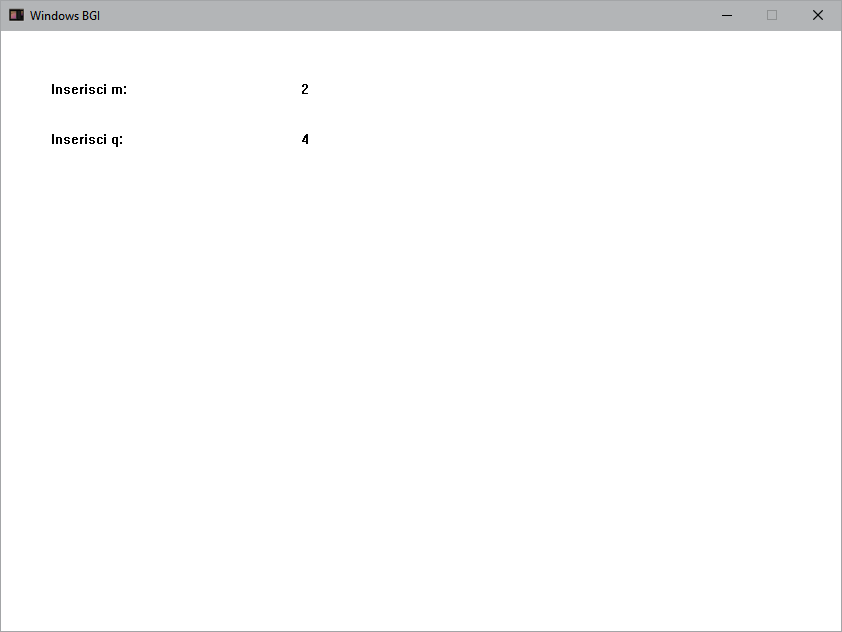
\includegraphics[scale=0.5]{tracciarettaterminale1}
						\\ \\
					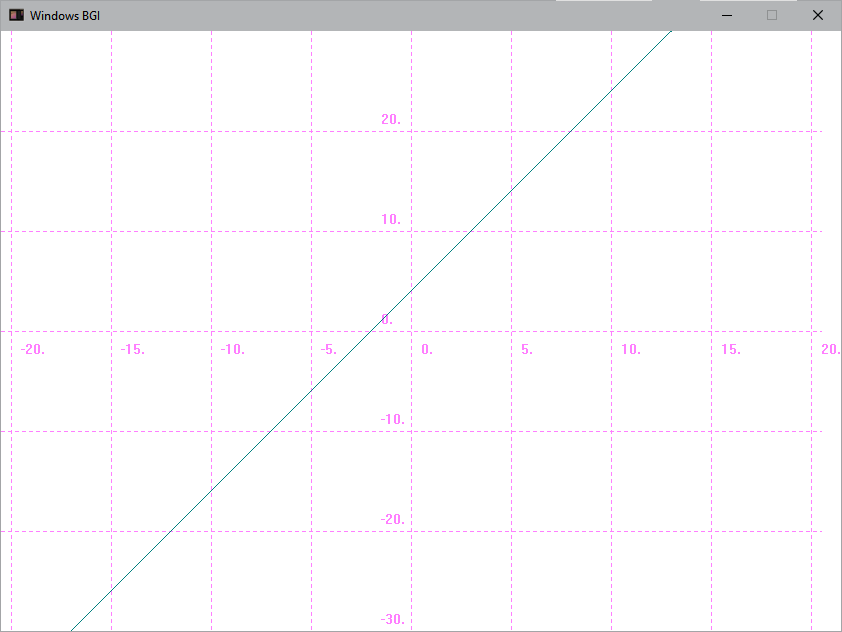
\includegraphics[scale=0.5]{tracciarettaterminale2}
				\end{figure*}
		\clearpage
			\newpage
%	------------------------------------------
		\clearpage
		\section{TracciaRettaVert}
		L'istruzione "tracciarettavert" viene usata per creare una linea verticale di pixel, di colore a scelta, per visualizzare una retta all'interno della finestra. Viene usata insieme al comando "assi" per creare grafici.
		\\La sintassi è la seguente:
		\\
		\\
		\Large tracciarettavert(x, rx, ry, col, center);
		\normalsize
		\\
		\\- x: indica lo spostamento rispetto all'asse y della retta da rappresentare (Offset);
		\\- rx: Il numero di parti in cui è diviso l'asse delle ascisse (Bisogna inserire lo stesso valore inserito nella funzione assi);
		\\- ry:Il numero di parti in cui è diviso l'asse delle ordinate(Bisogna inserire lo stesso valore inserito nella funzione assi);
		\\- col: indica il colore del pixel.
		\\- center: indica il centro del diagramma cartesiano disegnato con la funzione assi (Bisogna inserire lo stesso valore inserito nella funzione assi);
		\\
		\\Questo programma disegna una retta verticale su un diagramma cartesiano, dopo aver ottenuto l'offset tramite l'uso di "graphicScanfxy". Inoltre usa "cleardevice" per "ripulire" lo schermo.
		\\Codice e output:			
		\begin{lstlisting}
			{
			initwindow(850, 610);
			float x;
			
			outtextxy(50, 50, "Inserisci x:");
			graphicScanfxy(300, 50, "%f", &x);
			
			cleardevice();
			
			int rx, ry;
			rx = 40;
			ry = 60;
			assi(rx, ry, 1);
			
			tracciarettavert(x, rx, ry, 12, 1);
			getch();
			}
		\end{lstlisting}
		\begin{figure*}[h]
			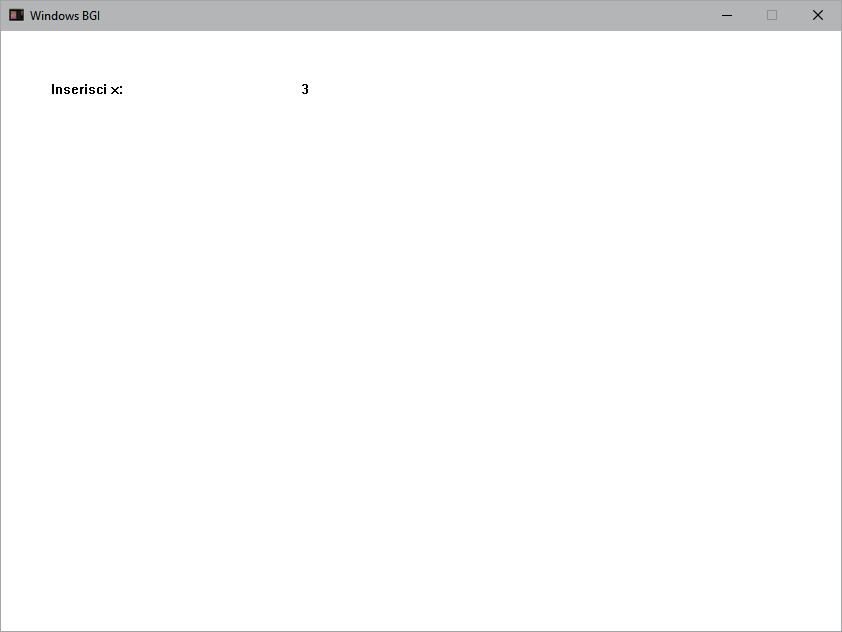
\includegraphics[scale=0.5]{tracciarettavertterminale1}
			\\ \\
			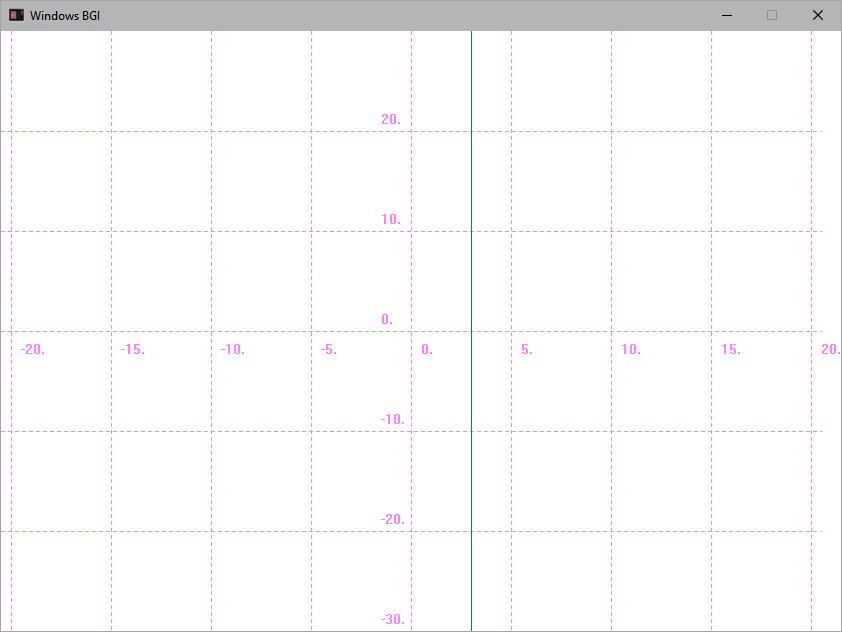
\includegraphics[scale=0.5]{tracciarettavertterminale2}
		\end{figure*}
		\clearpage
		\newpage
%	------------------------------------------
		\section{TracciaPunto}
			L'istruzione "tracciapunto" viene usata per disegnare un punto, di colore a scelta, all'interno della finestra. Il punto disegnato non è un singolo pixel, ma un piccolo cerchio. Viene  spesso usata per segnare un'intersezione o per rappresentare graficamente l'input dell'utente.
		\\La sintassi è la seguente:
		\\
		\\
		\Large tracciapunto(x, y, rx, ry, col, center);
		\normalsize
		\\
		\\- x: indica la coordinata x del punto da rappresentare;
		\\- y: indica la coordinata y del punto da rappresentare;
		\\- rx: Il numero di parti in cui è diviso l'asse delle ascisse (Bisogna inserire lo stesso valore inserito nella funzione assi);
		\\- ry:Il numero di parti in cui è diviso l'asse delle ordinate(Bisogna inserire lo stesso valore inserito nella funzione assi);
		\\- col: indica il colore del pixel.
		\\- center: indica il centro del diagramma cartesiano disegnato con la funzione assi (Bisogna inserire lo stesso valore inserito nella funzione assi);
		\\
		\\Questo programma disegna un punto su un diagramma cartesiano, dopo aver ottenuto le coordinate tramite l'uso di "graphicScanfxy".
		\\
		Codice e output:			
		\begin{lstlisting}
			{
				initwindow(850, 610);
				float x, y;

				outtextxy(50, 50, "Inserisci la x del punto:");
				graphicScanfxy(300, 50, "%f", &x);
				outtextxy(50, 100, "Inserisci la y del punto:");
				graphicScanfxy(300, 100, "%f", &y);
				cleardevice();

				int rx, ry;
				rx = 40;
				ry = 60;
				assi(rx, ry, 1);
				tracciapunto(x, y, rx, ry, 12, 1);
				getch();
			}
		\end{lstlisting}
		
		
		\begin{figure*}[h]
			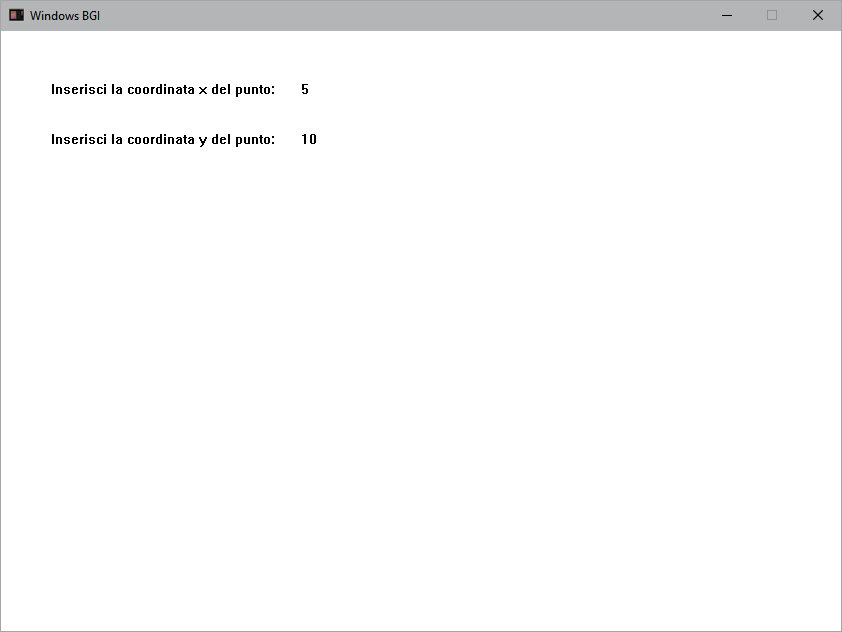
\includegraphics[scale=0.5]{tracciapuntoterminale1}
			\\ \\
			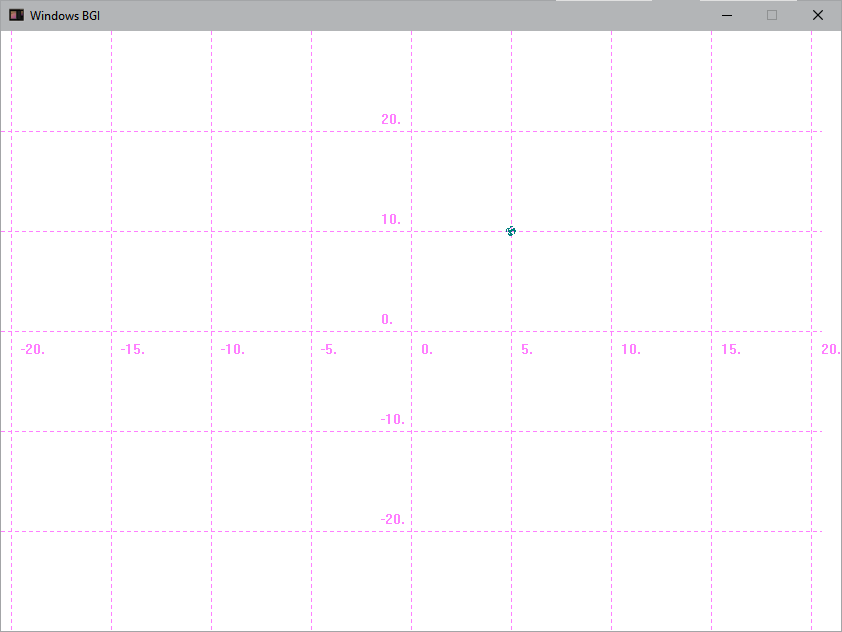
\includegraphics[scale=0.5]{tracciapuntoterminale2}
		\end{figure*}
		\clearpage
		\newpage
%	------------------------------------------
		\section{TracciaSegmento}
					L'istruzione "tracciasegmento" viene usata per tracciare un segmento, di colore a scelta, all'interno della finestra. Il segmento disegnato è quello che collega i punti A e B, inseriti nel comando. Può anche tracciare segmenti verticali.
		\\La sintassi è la seguente:
		\\
		\\
		\Large tracciasegmento(x1, y1, x2, y2, rx, ry, col, center);
		\normalsize
		\\
		\\- x1: indica la coordinata x del primo punto del segmento;
		\\- y1: indica la coordinata y del primo punto del segmento;
		\\- x2: indica la coordinata x del secondo punto del segmento;
		\\- y2: indica la coordinata y del secondo punto del segmento;
		\\- rx: Il numero di parti in cui è diviso l'asse delle ascisse (Bisogna inserire lo stesso valore inserito nella funzione assi);
		\\- ry:Il numero di parti in cui è diviso l'asse delle ordinate(Bisogna inserire lo stesso valore inserito nella funzione assi);
		\\- col: indica il colore del segmento.
		\\- center: indica il centro del diagramma cartesiano disegnato con la funzione assi (Bisogna inserire lo stesso valore inserito nella funzione assi);
		\\\\
		Questo programma disegna un segmento su un diagramma cartesiano, dopo aver ottenuto le coordinate tramite l'uso di "graphicScanfxy".
		\newpage
		Codice e output:			
		\begin{lstlisting}
		{
			initwindow(850, 610);
			float x1, y1, x2, y2;
			
			outtextxy(50, 50, "Inserisci la coord. x del punto 1:");
			graphicScanfxy(300, 50, "%f", &x1);
			outtextxy(50, 100, "Inserisci la coord. y del punto 1:");
			graphicScanfxy(300, 100, "%f", &y1);
			outtextxy(50, 150, "Inserisci la coord. x del punto 2:");
			graphicScanfxy(300, 150, "%f", &x2);
			outtextxy(50, 200, "Inserisci la coord. y del punto 2:");
			graphicScanfxy(300, 200, "%f", &y2);
			cleardevice();
			
			int rx, ry;
			rx = 40;
			ry = 60;
			assi(rx, ry, 1);
			
			tracciasegmento(x1, y1, x2, y2, rx, ry, 12, 1);
			getch();
		}
		\end{lstlisting}
	
		\newpage
		\begin{figure*}[h]
			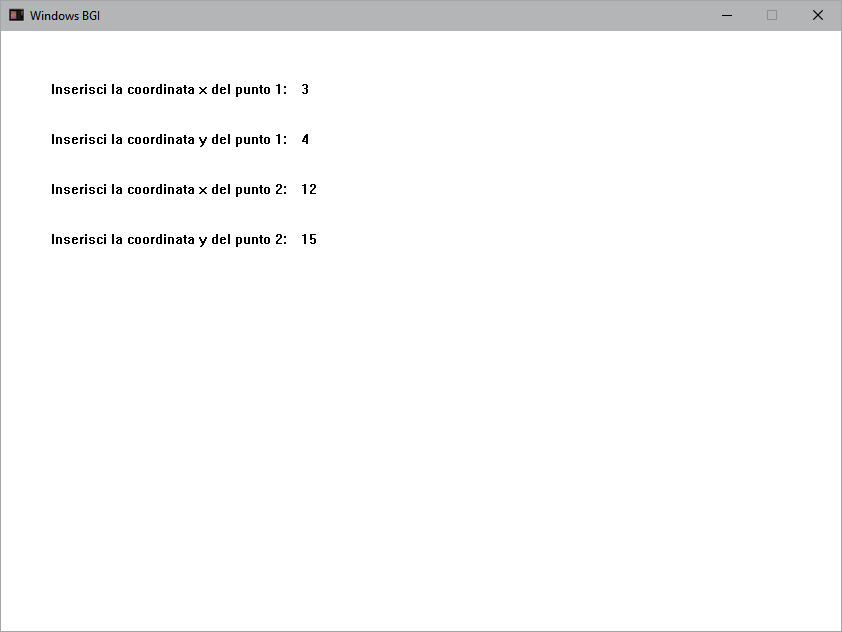
\includegraphics[scale=0.5]{tracciasegmentoterminale1}
\\ \\ 
			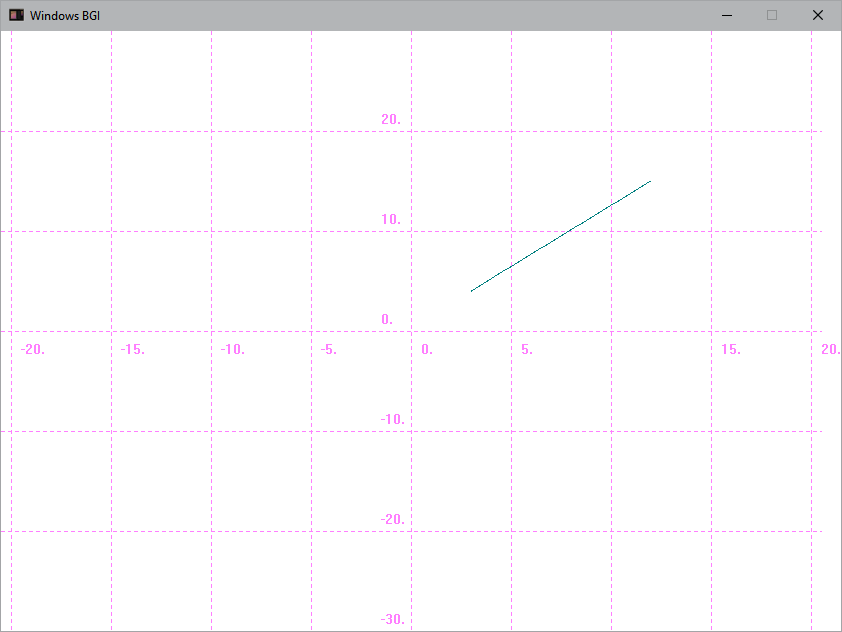
\includegraphics[scale=0.5]{tracciasegmentoterminale2}
		\end{figure*}
		\clearpage
		\newpage
%	------------------------------------------
		\section{TracciaCerchio}
			L'istruzione "tracciacerchio" viene usata per tracciare una circonferenza, di colore a scelta, all'interno della finestra.
			Quest'istruzione disegna una circonferenza data la sua equazione, mentre per disegnare un cerchio da raggio e coordinate del centro viene usato il comando "circle", compreso all'interno delle librerie standard del template "pino".
			\\
		\\La sintassi è la seguente:
		\\
		\\
		\Large tracciasegmento(a, b, c, rx, ry, col, center);
		\normalsize
		\\
		\\- a: indica il primo coefficiente dell'equazione della circonferenza (ax$^2$);
		\\- b: indica il secondo coefficiente dell'equazione della circonferenza (ax);
		\\- c: indica il terzo coefficiente dell'equazione della circonferenza; 
		\\- rx: Il numero di parti in cui è diviso l'asse delle ascisse (Bisogna inserire lo stesso valore inserito nella funzione assi);
		\\- ry:Il numero di parti in cui è diviso l'asse delle ordinate(Bisogna inserire lo stesso valore inserito nella funzione assi);
		\\- col: indica il colore del segmento.
		\\- center: indica il centro del diagramma cartesiano disegnato con la funzione assi (Bisogna inserire lo stesso valore inserito nella funzione assi);
		\\
		\\
		Questo programma disegna una circonferenza su un diagramma cartesiano, dopo aver ottenuto le coordinate tramite l'uso di "graphicScanfxy".
		\\\\Per far si che la circonferenza risulti effettivamente circolare, rx ed ry devono essere proporzionati in maniera tale che un unità sull'asse x abbia lo stesso numero di pixel di un unità nell'asse y. Per fare ciò, nel programma, ho impostato rx = 40 ed ry = 30. 
		\newpage
		Codice e output:			
		\begin{lstlisting}
			{
				initwindow(850, 610);
				float a,b,c;
				
				outtextxy(50, 50, "Inserisci il coefficiente a:");
				graphicScanfxy(300, 50, "%f", &a);
				outtextxy(50, 100, "Inserisci il coefficiente b:");
				graphicScanfxy(300, 100, "%f", &b);
				outtextxy(50, 150, "Inserisci il coefficiente c:");
				graphicScanfxy(300, 150, "%f", &c);
				cleardevice();
				
				int rx, ry;
				rx = 40;
				ry = 30;
				assi(rx, ry, 1);
				
				tracciacerchio(a, b, c, rx, ry, 14, 1);
				getch();
			}
		\end{lstlisting}
		
		
		\begin{figure*}[h]
			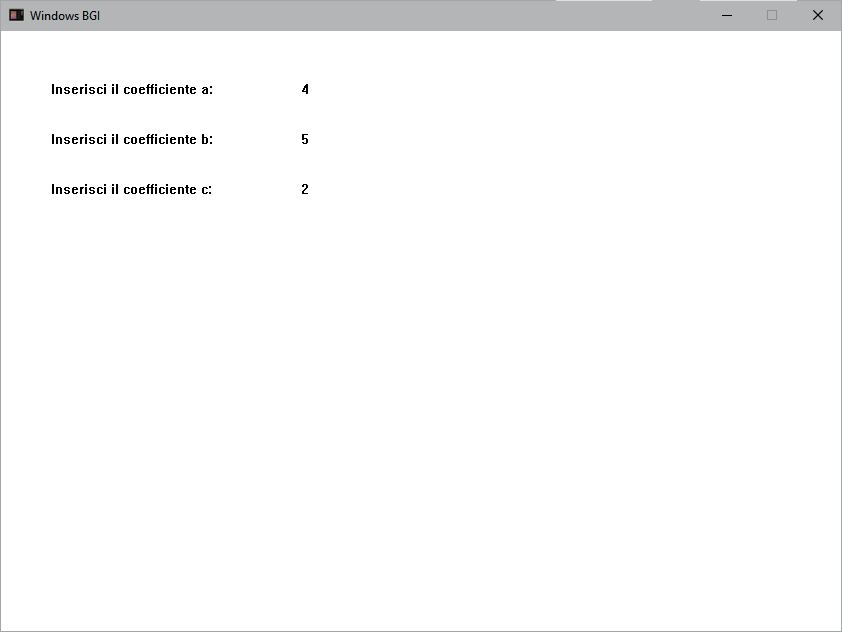
\includegraphics[scale=0.5]{tracciacerchioterminale1}
	\\ \\ 
			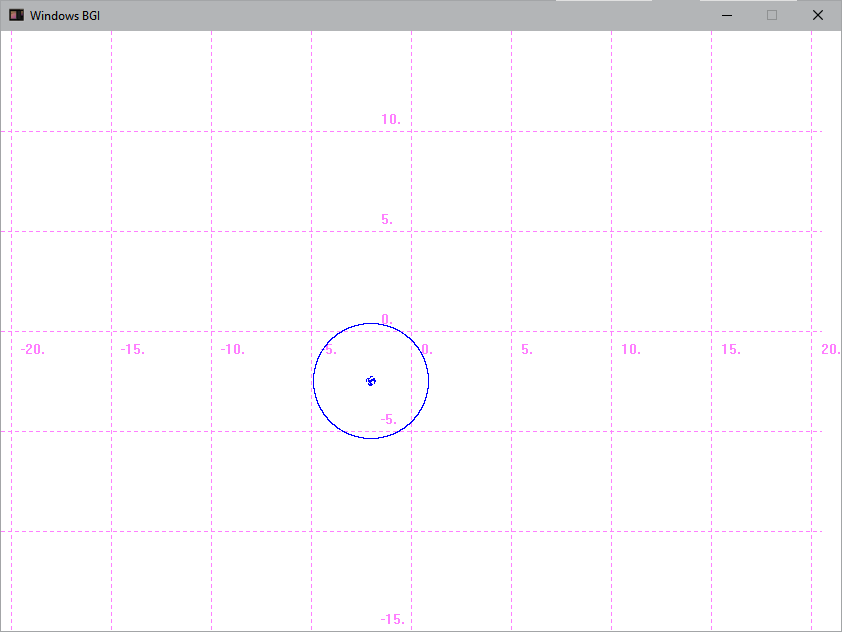
\includegraphics[scale=0.5]{tracciacerchioterminale2}
		\end{figure*}
		\clearpage
		\newpage
		\section{TracciaParabola}
	L'istruzione "tracciaparabola" viene usata per tracciare una parabola, di colore a scelta, all'interno della finestra.
	Quest'istruzione disegna una parabola data la sua equazione, che deve essere inserita in forma esplicita.
\\
\\La sintassi è la seguente:
\\
\\
\Large tracciaparabola(a, b, c, rx, ry, col, center);
\normalsize
\\
\\- a: indica il primo coefficiente dell'equazione della parabola (ax$^2$);
\\- b: indica il secondo coefficiente dell'equazione della parabola (ax);
\\- c: indica il terzo coefficiente dell'equazione della parabola; 
\\- rx: Il numero di parti in cui è diviso l'asse delle ascisse (Bisogna inserire lo stesso valore inserito nella funzione assi);
\\- ry:Il numero di parti in cui è diviso l'asse delle ordinate(Bisogna inserire lo stesso valore inserito nella funzione assi);
\\- col: indica il colore del segmento.
\\- center: indica il centro del diagramma cartesiano disegnato con la funzione assi (Bisogna inserire lo stesso valore inserito nella funzione assi);
\\
\\
Questo programma disegna una parabola su un diagramma cartesiano, dopo aver ottenuto le coordinate tramite l'uso di "graphicScanfxy".
\newpage
Codice e output:			
\begin{lstlisting}
	{
		initwindow(850, 610);
		float a,b,c;
		
		outtextxy(50, 50, "Inserisci il coefficiente a:");
		graphicScanfxy(300, 50, "%f", &a);
		outtextxy(50, 100, "Inserisci il coefficiente b:");
		graphicScanfxy(300, 100, "%f", &b);
		outtextxy(50, 150, "Inserisci il coefficiente c:");
		graphicScanfxy(300, 150, "%f", &c);
		
		cleardevice();
		
		int rx, ry;
		rx = 40;
		ry = 30;
		assi(rx, ry, 1);
		
		tracciaparabola(a, b, c, rx, ry, 14, 1);
		getch();
	}
\end{lstlisting}


\begin{figure*}[h]
	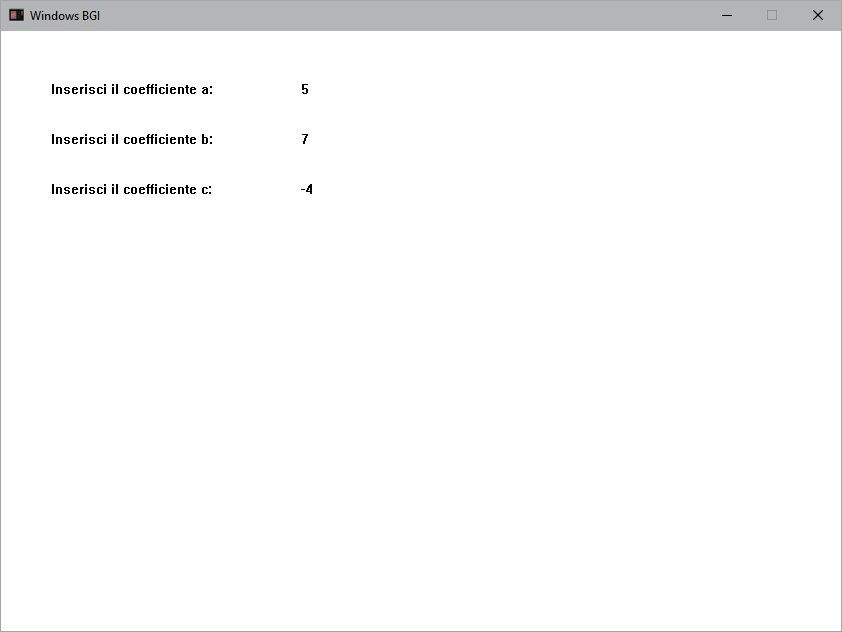
\includegraphics[scale=0.5]{tracciaparabolaterminale1}
 \\ \\ 
	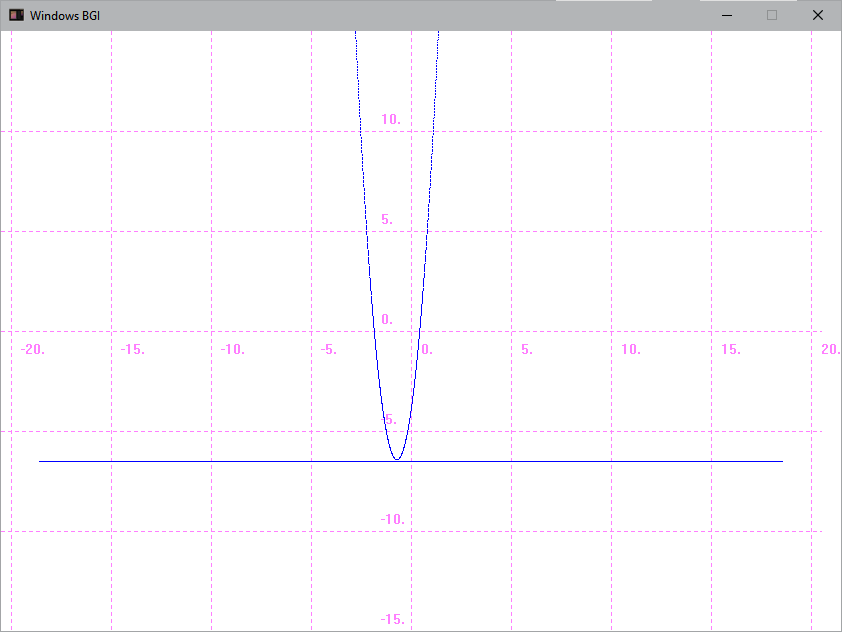
\includegraphics[scale=0.5]{tracciaparabolaterminale2}
\end{figure*}
\clearpage
\newpage
		\section{ScriviRetta}
			L'istruzione "scriviretta" viene viene usata per scrivere a schermo l'equazione di una retta.
			\\La sintassi è la seguente:
			\\
			\\
			\Large scriviretta(m, q, y);
			\normalsize
			\\
			\\- m: indica il coefficiente angolare della retta da scrivere;
			\\- q: indica la quota della retta da scrivere (il valore y con x=0);
			\\- y: la posizione del testo all'interno della pagina;
			\\
			\\Questo programma scrive l'equazione della retta, usando dati inseriti dall'utente, tramite l'uso dei comandi outtextxy e graphicScanfxy.
			\\
			\\Codice e output:
			\begin{lstlisting}
				{
					initwindow(850, 610);
					float m, y, q;
					y = 150;

					outtextxy(50, 50, "Inserisci m:");
					graphicScanfxy(300, 50, "%f", &m);

					outtextxy(50, 100, "Inserisci q:");
					graphicScanfxy(300, 100, "%f", &q);

					scriviretta(m, q, y)
					getch();
				}
			\end{lstlisting}
			\begin{figure}[h]
				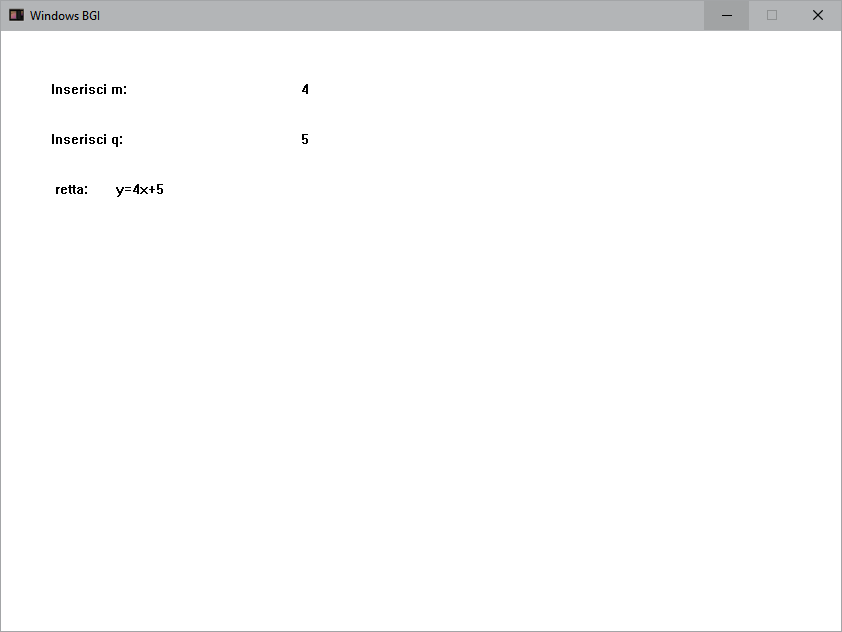
\includegraphics[scale=0.5]{scrivirettaterminale1}
			\end{figure}
		\clearpage
%	------------------------------------------
		\section{ScriviRettaVert}
					L'istruzione "scrivirettavert" viene viene usata per scrivere a schermo l'equazione di una retta verticale.
		\\La sintassi è la seguente:
		\\
		\\
		\Large scrivirettavert(x ,y);
		\normalsize
		\\
		\\- x: indica il valore x della retta da scrivere;
		\\- y: l'altezza del testo all'interno della finestra;
		\\
		\\Questo programma scrive l'equazione di una retta verticale, usando dati inseriti dall'utente, tramite l'uso dei comandi outtextxy e graphicScanfxy.
		\\ \\ \\
		Codice e output:
		\begin{lstlisting}
			{
				initwindow(850, 610);
				float x, y;
				y = 150;
				
				outtextxy(50, 50, "Inserisci x:");
				graphicScanfxy(300, 50, "%f", &x);

				scrivirettavert(x, y);
				getch();
			}
		\end{lstlisting}
		
		\begin{figure}[h]
			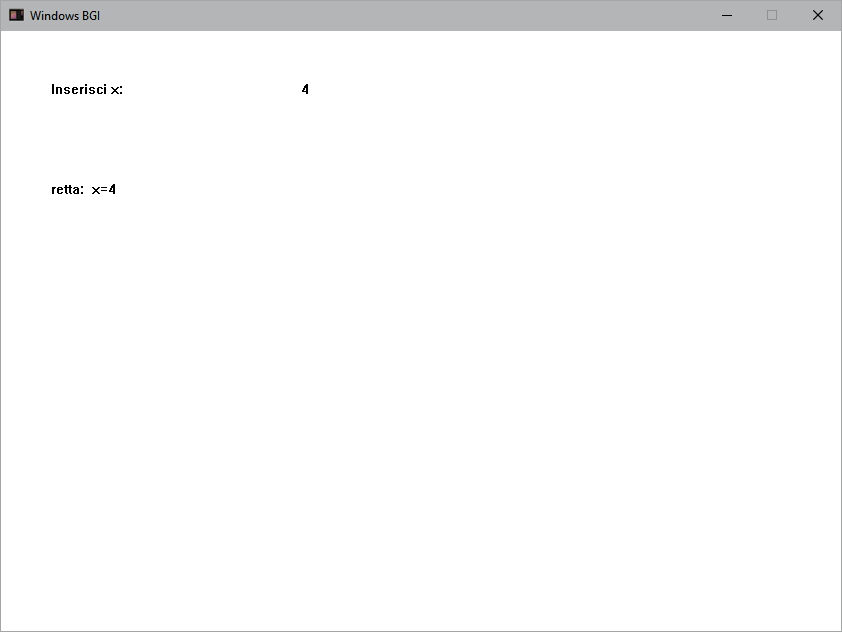
\includegraphics[scale=0.5]{scrivirettavertterminale1}
		\end{figure}
		\clearpage
%	------------------------------------------
		\section{ScriviCerchio}
		L'istruzione "scrivicerchio" viene viene usata per scrivere a schermo l'equazione di una circonferenza.
		\\La sintassi è la seguente:
		\\
		\\
		\Large scrivicerchio(a, b, c, y);
		\normalsize
		\\
		\\- a: indica il primo coefficiente dell'equazione della circonferenza (ax$^2$);
		\\- b: indica il secondo coefficiente dell'equazione della circonferenza (ax);
		\\- c: indica il terzo coefficiente dell'equazione della circonferenza; 
		\\- y: la posizione del testo all'interno della pagina;
		\\
		\\Questo programma scrive l'equazione di una circonferenza, usando dati inseriti dall'utente, tramite l'uso dei comandi outtextxy e graphicScanfxy.
		\\ \\ \\
		Codice e output:
		\begin{lstlisting}
			{
				initwindow(850, 610);
				float a, b, c, y;
				y = 250;
				
				outtextxy(50, 50, "Inserisci a:");
				graphicScanfxy(300, 100, "%f", &a);
				outtextxy(50, 100, "Inserisci b:");
				graphicScanfxy(300, 150, "%f", &b);
				outtextxy(50, 50, "Inserisci c:");
				graphicScanfxy(300, 150, "%f", &c);
				
				scrivicerchio(a, b, c, y);
				getch();
			}
		\end{lstlisting}
	
		\begin{figure}[h]
			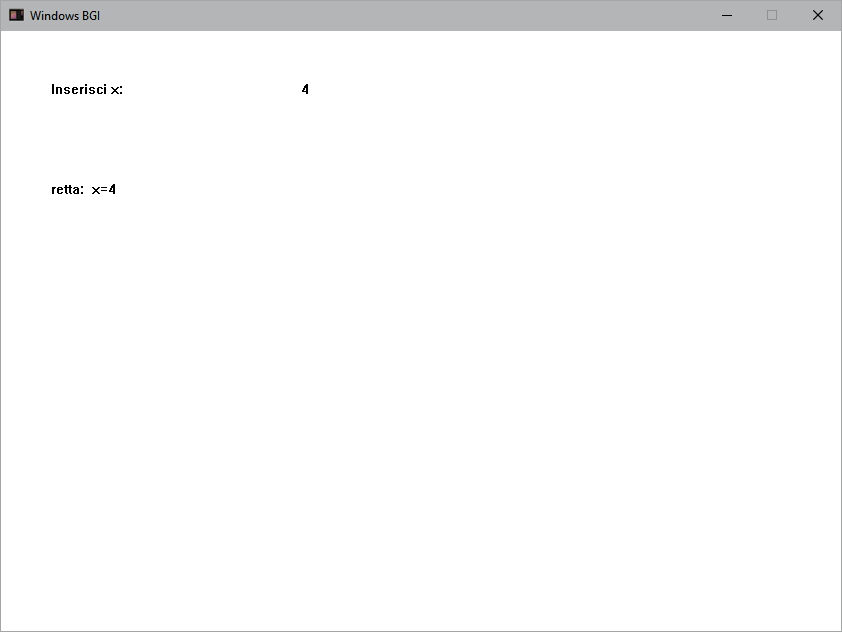
\includegraphics[scale=0.5]{scrivirettavertterminale1}
		\end{figure}
		\clearpage
%	------------------------------------------
		\section{ScriviParabola}
		L'istruzione "scriviparabola" viene viene usata per scrivere a schermo l'equazione di una parabola.
		\\La sintassi è la seguente:
		\\
		\\
		\Large scriviparabola(a, b, c, y);
		\normalsize
		\\
		\\- a: indica il primo coefficiente dell'equazione della parabola (ax$^2$);
		\\- b: indica il secondo coefficiente dell'equazione della parabola (ax);
		\\- c: indica il terzo coefficiente dell'equazione della parabola; 
		\\- y: la posizione del testo all'interno della pagina;
		\\
		\\Questo programma scrive l'equazione di una parabola, usando dati inseriti dall'utente, tramite l'uso dei comandi outtextxy e graphicScanfxy.
		\\ \\Codice e output:
		\begin{lstlisting}
			{
				initwindow(850, 610);
				float a, b, c, y;
				y = 250;
				
				outtextxy(50, 50, "Inserisci a:");
				graphicScanfxy(300, 50, "%f", &a);
				outtextxy(50, 100, "Inserisci b:");
				graphicScanfxy(300, 100, "%f", &b);
				outtextxy(50, 150, "Inserisci c:");
				graphicScanfxy(300, 150, "%f", &c);
				
				scriviparabola(a, b, c, y);
				getch();
			}
		\end{lstlisting}
		

		\begin{figure}[h]
			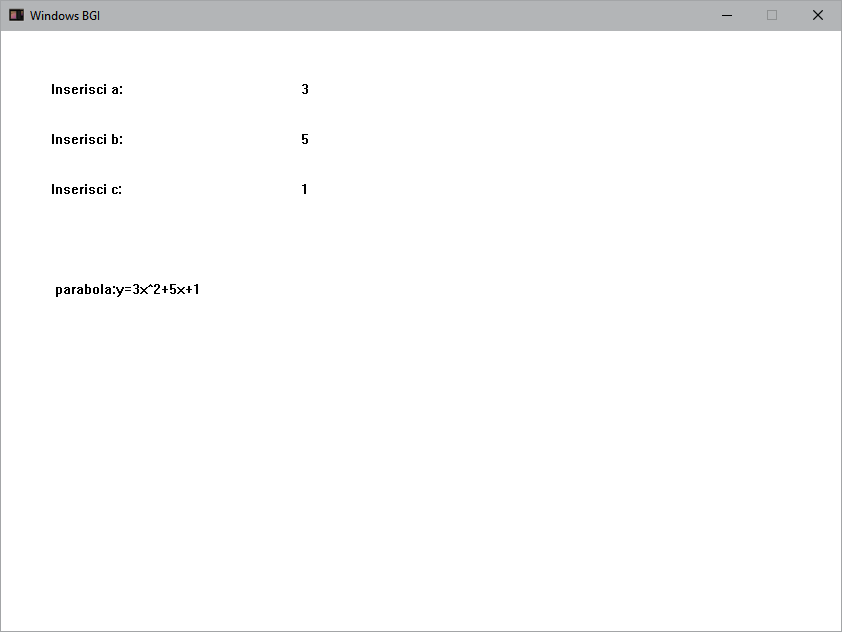
\includegraphics[scale=0.5]{scriviparabolaterminale1}
		\end{figure}
		\clearpage

		\section{ScriviEllisse}
		L'istruzione "scriviellisse" viene viene usata per scrivere a schermo l'equazione di un ellisse.
		\\La sintassi è la seguente:
		\\
		\\
		\Large scriviparabola(a, b, y);
		\normalsize
		\\
		\\- a: indica il primo coefficiente dell'equazione dell'ellisse (ax$^2$);
		\\- b: indica il secondo coefficiente dell'equazione dell'ellisse (ax);
		\\- y: la posizione del testo all'interno della pagina;
		\\
		\\Questo programma scrive l'equazione di una parabola, usando dati inseriti dall'utente, tramite l'uso dei comandi outtextxy e graphicScanfxy.
		Codice: e output:
		\begin{lstlisting}
			{
				initwindow(850, 610);
				float a, b, y;
				y = 200;
				
				outtextxy(50, 50, "Inserisci a:");
				graphicScanfxy(300, 50, "%f", &a);
				outtextxy(50, 100, "Inserisci b:");
				graphicScanfxy(300, 100, "%f", &b);
				
				scriviellisse(a, b, y);
				getch();
			}
		\end{lstlisting}
	
		\begin{figure}[h]
			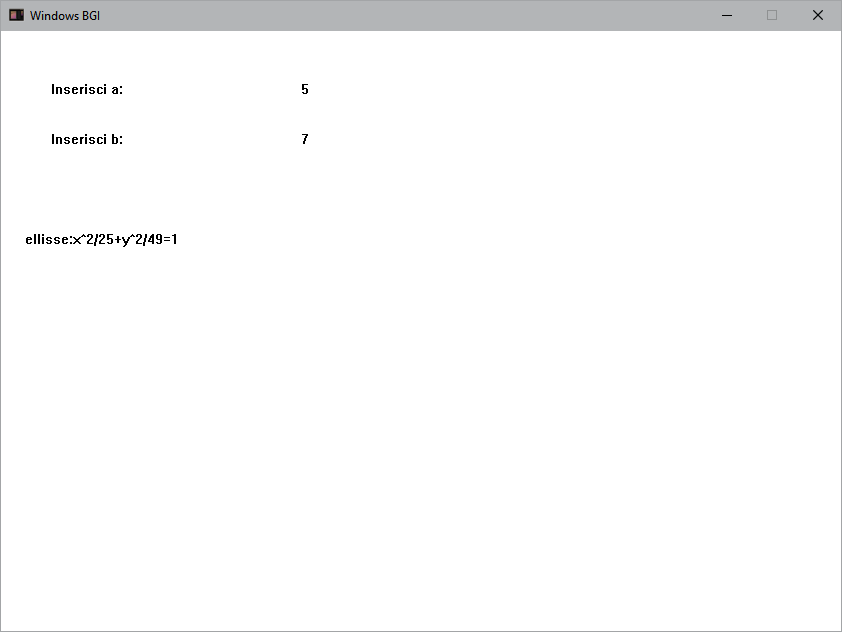
\includegraphics[scale=0.5]{scriviellisseterminale1}
		\end{figure}
		\clearpage


%	------------------------------------------

		
	
	
	
\end{document}	